\documentclass[12pt]{ctexart} % 文章类型为article,或者为paper等,ctexart为支持中文的article
% article 文章格式的文档类,广泛用于科技论文、报告、说明文档等。
% report 长篇报告格式的文档类,具有章节结构,用于综述、长篇论文、简单的书籍等。
% book 书籍文档类,包含章节结构和前言、正文、后记等结构。
% proc 基于 article 文档类的一个简单的学术文档模板。
% slides 幻灯格式的文档类,使用无衬线字体。
% minimal 一个极其精简的文档类,只设定了纸张大小和字号,用作代码测试的最小工作示例
% (Minimal Working Example)。
%10pt, 11pt, 12pt 指定文档的基本字号。缺省为 10pt。
\usepackage{newtxtext,newtxmath} % 数学公式
\usepackage{graphicx} % 插入图片
\usepackage{subfig}%子图
\DeclareGraphicsExtensions{.eps,.mps,.pdf,.jpg,.png}%指定图片后缀列表,让TEX自行查找;
\DeclareGraphicsRule{*}{png}{*}{}%告诉 LATEX 未知后缀的都是png
\usepackage{palatino}%绘制流程图
\usepackage{amsmath}%数学公式
\usepackage{tikz}%绘制流程图
\usetikzlibrary{shapes.geometric, arrows}%绘制流程图
\usepackage{booktabs}%三线表
\usepackage{longtable}%长表格
% 如需要特殊功能则引用其他必需的包
\usepackage{cite} % 引用文献

\usepackage{bm} % 粗体
\usepackage[colorlinks , allcolors=blue]{hyperref}%超链接
\hypersetup{colorlinks=true,linkcolor=black}
% “colorlinks”的意思是将超链接以颜色来标识,而并非使用默认的方框来标识。linkcolor, anchorcolor, citecolor分别表示用来标识link, anchor, cite等各种链接的颜色。若正式的文档中不想使用彩色的标识,但又希望具有超链接的功能,则将上例中的各种颜色换成“black”即可。
\usepackage[cache=false]{minted}  % 代码高亮
% \usepackage{ctex}%支持中文
% \usepackage{xeCJK}
\usepackage{fontspec}%字体设置
\setmainfont{Times New Roman}%表示为设置默认英文字体为Times New Roman.
%表示为设置默认英文字体为Times New Roman.
\usepackage{xcolor}% 指定颜色的text

\usepackage{indentfirst}%首段缩进
\setlength{\parindent}{2em}%首段缩进两个字符
\usepackage{setspace}%目录内标题行间距

\setcounter{secnumdepth}{4}%设置\paragraph的目录深度为4
\setcounter{tocdepth}{4}%设置\paragraph的编号深度为4

\usepackage{zhnumber} % change section number to chinese
\renewcommand\thesection{\zhnum{section}}
\renewcommand\thesubsection{\arabic{section}.\arabic{subsection}}



\begin{document} % 开始
\pagestyle{plain}%设置页眉页脚。plain为页眉为空,页脚为页码。(article 和 report 文档类默认;book文档类的每章第一页也为 plain 格式)
\title{Title} % 标题
\author{Author--WangziYao} % 作者
\date{March 2022}
\maketitle % 使标题和作者显示,必须要有

\thispagestyle{empty} % 去掉本页页码
\newpage % 开启下一页
\pagenumbering{Roman} % 从此开始到下次重新声明为止的页码编号数字为罗马数字
% arabic: arabic numerals
% roman: lowercase roman numerals
% Roman: uppercase roman numerals
% alph: lowercase letters
% Alph: uppercase letters


\begin{spacing}{1}%设置目录内标题行间距
\tableofcontents % 生成文章目录
\end{spacing}

\newpage % 开启下一页
\listoffigures % 生成图片目录
\newpage % 开启下一页
\listoftables % 生成表格目录
\newpage % 开启下一页

\pagenumbering{arabic}%从此开始到下次重新声明为止的页码编号数字为阿拉伯数字

\begin{abstract}
该部分内容是放置摘要信息的。该部分内容是放置摘要信息的。该部分内容是放置摘要信息的。该部分内容是放置摘要信息的。该部分内容是放置摘要信息的。
\end{abstract}
\newpage

\section{一级标题} % 一级标题
\href{http://t.csdn.cn/iGyt7}{latex安装与配置}

texlive环境+texstudio编译器
\subsection{二级标题} % 二级标题

During

\indent line% 缩进
\par new line% or

\noindent Thirty-two line.% 不缩进
new line\footnote{content}

\subsubsection{三级标题} % 三级标题
\begin{table}[htbp]
    \caption{字号转换}
    \centering
    \begin{tabular}{|l|l|}
    \hline
        初号字  & 42pt  \\ \hline
        小初号字 & 36pt  \\ \hline
        一号字 & 26pt  \\ \hline
        小一号字 & 24pt  \\ \hline
        二号字 & 22pt  \\ \hline
        小二号字 & 18pt  \\ \hline
        三号字 & 16pt  \\ \hline
        小三号字 & 15pt  \\ \hline
        四号字 & 14pt  \\ \hline
        小四号字 & 12pt  \\ \hline
        五号字 & 10.5pt  \\ \hline
        小五号字 & 9pt  \\ \hline
        六号字 & 7.5pt  \\ \hline
        小六号字 & 6.5pt  \\ \hline
        七号字 & 5.5pt  \\ \hline
        八号字 & 5pt \\ \hline
    \end{tabular}
\end{table}

\paragraph{伪四级标题} % 无编号段落标题
\begin{itemize}%用实心圆点符号对文本排序
    \item item 1
    \item item 2
    \item item 3
\end{itemize}
\begin{enumerate}%用数字编号对文本排序
    \item item 1
    \item item 2
    \item item 3
\end{enumerate}

% 正文
\section{正文}
	\heiti 你好\par
	\kaishu 到目前为止,你已经可以用LaTeX自带的article模板来书写一篇基本的论文框架了,至少你已经能够借助搜索然后复制粘贴这些命令例子来开始用LaTeX编辑了 
	
	\fangsong 在论文从框架到完整的过程中,必然还存在许多的细节问题,比如字体字号,比如图片拼合,比如复杂的表格等等。 

	\begin{center}
	\vspace{-0.8em}%在垂直段落产生-0.8em的长度
    本\hspace{1em}段\hspace{1em}落\hspace{1em}居\hspace{1em}中\\%水平产生一个字符的间距
	那些问题,就请咨询google吧。通常来说我们作为初学者会提出的问题,早就已经有许多的先辈们在网络上提过同样的问题了,看看别人的回答就可以
	\vspace{-0.8em}%在垂直段落产生-0.8em的长度
    \end{center}
	那些问题,就请咨询google吧。通常来说我们作为初学者会提出的问题,早就已经有许多的先辈们在网络上提过同样的问题了,看看别人的回答就可以。
	 
	LaTeX在国内的普及率并不高,因此许多时候如果搜英文关键词,会获得更好的效果。

	\LaTeX
	\newpage
    %字体族设置(罗马字体、无衬线字体、打印机字体)
     \textrm{Roman Family} \textsf{Sans Serif Family} \texttt{Typewriter Family}    
     {\rmfamily Roman Family} {\sffamily Sans Serif Family} {\ttfamily Typewriter Family}
     {\sffamily who you are? you find self on everyone around. take you as the same as others!}
     {\ttfamily Are you wiser than others? definitely on. in some days, my it is true. What can you achieve? a luxurious house? a brillilant car? an admirable career? who knows?}
     
     %字体系列设置(粗细、宽度)
     \textmd{Medium Series} \textbf{Boldface Series}
     {\mdseries Medium Series} {\bfseries Boldface Series}
     
     %字体形状(直立、斜体、伪斜体、小型大写)
     \textup{Upright Shape} \textit{Italic Shape} \textsl{Slanted Shape} \textsc{Small Caps Shape}
     
     {\upshape Upright Shape} {\itshape Italic Shape} {\slshape Slanted Shape} {\scshape Small Caps Shape}
     
     %中文字体
     {\songti 宋体} \quad {\heiti 黑体} \quad {\fangsong 仿宋} \quad {\kaishu 楷书}
     中文字体的 \textbf{粗体} 和 \textit{斜体} 。
     
     %字体大小,根据normalsize的大小确定,normalsize 在文档类的参数决定
     {\tiny           Hello}\par
     {\scriptsize     Hello}\\
     {\footnotesize   Hello}\\
     {\small          Hello}\\
     {\normalsize      Hello}\\
     {\large          Hello}\\
     {\Large          Hello}\\
     {\LARGE          Hello}\\
     {\huge           Hello}\\     
     {\Huge           Hello}\\     
     %中文字号设置命令、
     \zihao{-0} 你好!%12pt
     
     \zihao{5} 你好!
     
\section{特殊字符}
\# \$ \% \^{} \& \_ \{ \} \~{} \textbackslash

\section{数学}
正文$E = mc^2$%内嵌公式
$$E = mc^2$$%公式居中

\begin{equation}
E=mc^2
\end{equation}

\[ E=mc^2 \]
%\[ same as \begin{displaymath} or $$.
%\] same as \end{displaymath} or $$.
\[ \boxed{E=mc^2} \]

\begin{align}
    E = mc^2
\end{align}

\subsection{指数、下标、根号}
\subsubsection{指数、上下标、根号}
\[x_{ij}^2\quad \sqrt[3]{x}\]
$ x_i^3 \sqrt{x} $
\[x_{\text{下标}}^{\text{上标}} \]

\subsubsection{分数}
$\frac{1}{2}$ \quad $ \dfrac{1}{2}$ \quad $ \tfrac{1}{2}$
% 分数用 \frac 命令表示,它会自动调整字号,比如在行间公式中小一点,在独立公式则大一点。
% \dfrac 命令把分数的字号显式设置为独立公式中的大小,\tfrac 命令则把字号设为行间公式中的大小
\subsection{运算符}

\[\pm \times \div\] 
\[\cdot \cap \cup\] 
\[ \geq \leq \neq \] 
\[\approx \equiv\]

$$
\left\{\begin{array}{c}
x(t)=\displaystyle \sum_{n=-\infty}^{\infty} \boldsymbol{X}(n \Omega) e^{j n \Omega t} \\
\boldsymbol{X}(n \Omega)=\frac{1}{T} \int_{t}^{t+\mathrm{T}} x(t) e^{-j n \Omega t} d t
\end{array}\right.
$$

$ \sum_{i=1}^n i \prod_{i=1}^n \lim_{x\to0}x^2 \int_a^b x^2 dx $
$$ \sum_{i=1}^n i \prod_{i=1}^n \lim_{x\to0}x^2 \int_a^b x^2 dx $$
\[ \sum_{i=1}^n i \prod_{i=1}^n \lim_{x\to0}x^2 \int_a^b x^2 dx \]
\[
P = \frac
{\sum_{i=1}^n (x_i- x)(y_i- y)}
{\displaystyle \left[
\sum_{i=1}^n (x_i-x)^2
\sum_{i=1}^n (y_i-y)^2
\right]^{1/2} }
\]

\begin{figure}[htbp]
\centering
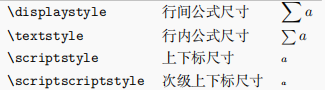
\includegraphics[scale=0.7]{figures/chicun.png}
	\caption{数学公式行内尺寸}
	\label{fig:chicun}
\end{figure}

\subsubsection{多重积分符号}
 $ \int x dx \iint x dx \iiint x dx \iiiint x dx \idotsint x dx $
 
\begin{figure}[htbp]
\centering
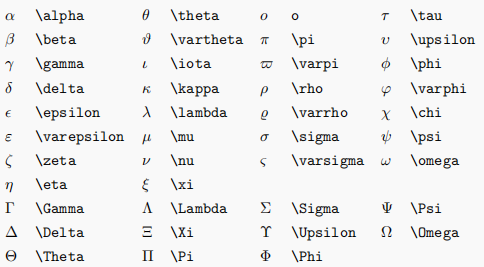
\includegraphics[scale=0.7]{figures/fuhao}
	\caption{数学符号说明}
	\label{fig:fuhao}
\end{figure}
	
 \subsection{标注}
$$\acute{x}  \tilde{x}  \mathring{x}$$
$$ \grave{x}  \breve{x}  \dot{x}$$
$$\bar{x}  \check{x}  \ddot{x}$$
$$ \vec{x}  \hat{x}  \dddot{x} $$
\subsection{省略}
\[ \dots \cdots \vdots \ddots \]

\subsection{公式}
\href{https://www.mathtype.cn/jiqiao/gongshi-daima.html}{latex to mathtype}

\begin{multline}%公式一行放不下
x=a+b+c+d+e+f+g+h+i+j+k+\\ l+m+n+o+p+q+r+s+t+u+v+w+x+y+z
\end{multline} %多行不需要对齐的长公式

\begin{equation}
    \begin{split}%多行需要对齐的长公式
    x=&a+b+c+d+e+f+g+h+i+j+k+\\ &l+m+n+o+p+q+r+s+t+u+v+w+x+y+z
    \end{split}
\end{equation}

\begin{align}%多行公式靠右对齐,多行公式只有一个编号
    \begin{aligned}
        E = \frac{1}{2}mv^2 \\
        x = v_{0}t + \frac{1}{2}at^{2}
    \end{aligned}
\end{align}

\begin{align}%多行公式靠左对齐,多行公式多个编号
        E &= \frac{1}{2}mv^2 \\
        x &= v_{0}t + \frac{1}{2}at^{2}
\end{align}

\begin{gather}%居中对齐多个编号
    E = \frac{1}{2}mv^2 \\
    v = v_{0}t + \frac{1}{2}at^{2}
\end{gather}

\subsection{矩阵}
\[\begin{array}{ccc}
%参数 {ccc} 用于设置每列的对齐方式,l、c、r 分别表示左中右;\\ 和 & 用来分隔行和列。
~ & x_2 & \dots \\
x_3 & x_4 & \dots \\
\vdots & \vdots & \ddots \\
\end{array}\]
%pmatrix、bmatrix、Bmatrix、vmatrix和Vmatrix,它们和 array 的主要区别是会在表两端加上 () [] {} || kk 等分隔符,其次这些环境没有列对齐方式参数。

\begin{align}
    \left[
    \begin{array}{lcr} % c为居中对齐,l为左对齐,r为右对齐
        11&0&0 \\
        0&222&0 \\
        0&0&3333
    \end{array}
    \right]
\end{align}

\[
\begin{matrix}
1 & 2 \\
3 & 4
\end{matrix} \qquad
\begin{bmatrix}
p_{11} & p_{12} & \ldots & p_{1n} \\
p_{21} & p_{22} & \ldots & p_{2n} \\
\vdots & \vdots & \ddots & \vdots \\
p_{m1} & p_{m2} & \ldots & p_{mn}
\end{bmatrix}
\]

\begin{align}%矩阵
    \begin{aligned}
        y = \left( \frac{a}{b} \right) \\
        y = \left( \frac{a}{b} \right. \\
        y = (\frac{a}{b})
    \end{aligned}
\end{align}

\[
\mathbf{X} = \left(
\begin{array}{ccc}
x_1 & x_2 & \ldots \\
x_3 & x_4 & \ldots \\
\vdots & \vdots & \ddots
\end{array} \right)
\]

\begin{align}%中括号
    f(x) =\left\{
        \begin{aligned}
        0~, \qquad x<0 \\ % 使用 ~ 作为小空格
        1~, \qquad x>0
        \end{aligned} 
        \right.
\end{align}
\[
|x| = \left\{
\begin{array}{rl}
-x & \text{if } x < 0,\\
0 & \text{if } x = 0,\\
x & \text{if } x > 0.
\end{array} \right.
\]

\begin{align}%在想让其对齐的位置前加 & 以等号对齐为例
    \begin{aligned}
        f(x) &= \frac{2}{4} \\
        & = \frac{1}{2}
    \end{aligned} 
\end{align}

\section{图片大关}
\subsection{插图}
scale 缩放比例
width 宽度
height 高度
totalheight 范围框高度,旋转时它不等于高度
keepaspectratio 如果不使用它而同时指定插图的宽度、高度,长宽比
可能会失调;使用它时长宽比不变,宽度、高度都不
超过指定参数
angle 旋转角度
origin 旋转原点

viewport 可视区域的左上角和右下角坐标。
trim 左、下、右、上四边裁剪的数值。
clip 是否真正裁剪。缺省为false,不执行裁剪,多出的部分就那样放着;设置为true时执行裁剪。似乎是多此一举。

\begin{figure}[htbp]%位置选项
\centering
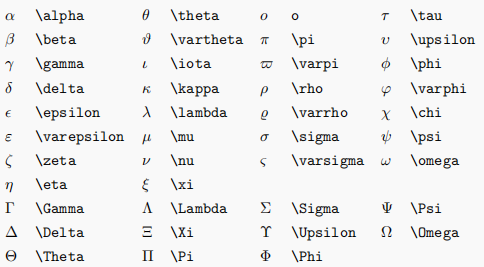
\includegraphics[bb=0 0 410 307,scale=.6]{figures/fuhao.png}
\caption{符号}
\label{fig:fu}
\end{figure}

[htbp] 选项用来指定插图排版的理想位置,这几个字\ref{fig:fu}
母分别代表 here、top、bottom、float page,也就是固定位置、页顶、页尾、单独的浮动页
%\centering 用来使插图居中
%label 应放在caption 之后,否则用时指向的是前一个插图

\begin{figure}[h]
\centering

\includegraphics[scale=.5]{figures/off.png}

\includegraphics[scale=0.5]{figures/on.png}
\caption{开关灯}
\end{figure}

\begin{figure}[htbp]
\centering
\begin{minipage}[b]{.3\textwidth}
\centering

\includegraphics[scale=0.5]{figures/off.png}
\caption{关灯}
\end{minipage}
\begin{minipage}[b]{.3\textwidth}
\centering

\includegraphics[scale=0.5]{figures/on.png}
\caption{开灯}
\end{minipage}
\end{figure}

\noindent \textbackslash linewidth - 当前行的宽度\\
\textbackslash columnwidth - 当前栏的宽度 (看清是单栏还是双栏)\\
\textbackslash textwidth - 整个页面版面的宽度 (文字区域)\\
\textbackslash paperwidth - 整个页面纸张的宽度 (整个纸)\\

\begin{figure}[htbp]
\centering
\subfloat[关灯]{
\label{fig:subfig_a}

\includegraphics[scale=0.5]{figures/off.png}
}
\hspace{10pt}
\subfloat[开灯]{
\label{fig:subfig_b}

\includegraphics[scale=0.5]{figures/on.png}
}
\caption{开关灯}
\end{figure}

\begin{figure}[htbp]
\centering
\subfloat[关灯]{
\label{fig:improved_subfig_a}
\begin{minipage}[t]{0.3\textwidth}
\centering

\includegraphics[scale=0.5]{figures/off.png}
\end{minipage}
}
\subfloat[开灯]{
\label{fig:improved_subfig_b}
\begin{minipage}[t]{0.3\textwidth}
\centering

\includegraphics[scale=0.5]{figures/on.png}
\end{minipage}
}
\caption{开关灯}
\end{figure}

\subsection{绘制流程图}
% 流程图定义基本形状
\tikzstyle{startstop} = [rectangle, rounded corners, minimum width = 2cm, minimum height=1cm,text centered, draw = green, fill = red!40]
\tikzstyle{io} = [trapezium, trapezium left angle=70, trapezium right angle=110, minimum width=2cm, minimum height=1cm, text centered, draw=black, fill = blue!40]
\tikzstyle{process} = [rectangle, minimum width=3cm, minimum height=1cm, text centered, draw=black, fill = yellow!50]
\tikzstyle{decision} = [diamond, aspect = 3, text centered, draw=black, fill = green!30]
% 箭头形式
\tikzstyle{arrow} = [->,>=stealth]

\begin{tikzpicture}[node distance=3cm]%由于之前process最小宽度较大,故而会产生重合
\tikzstyle{every node}=[font=\small,scale=0.8]
\node(1)[startstop]{1};
\node(2)[process,below of =1]{2};
\node(3)[io,left of=2]{4};
\node(4)[startstop,below of =3]{1};
\draw[arrow] (1)--(2);
\draw[arrow] (1)--(2);
\draw[arrow] (2)|-(4);
\end{tikzpicture}

\begin{tikzpicture}[node distance=1.5cm]
\tikzstyle{every node}=[font=\small,scale=0.8]
%定义流程图具体形状
\node (start) [startstop]
{Start};
\node (in1) [io, below of = start]
{Initial $x_0=(x_{01},x_{02},\cdots)$};
\node (pro1) [process, right of = in1, xshift = 5cm]
{Calculation $u_0=f(x_0)$};
\node (pro4) [process, below of = in1]
{New result $u^*=f(x_0^*)$};
\node (pro3) [process, below of=pro1]
{New solution $x_0^*=(\cdots,x_{0i},\cdots$)};
\node (pro2) [process, right of=pro3, xshift = 4cm]
{Randomly change $x_0$ into $x_0^*$};
\node (dec1) [decision, below of=pro4]
{Optimized?};
\node (pro5) [process, below of=pro3]
{Accept new solution probobly};
\node (pro6) [process, below of=dec1]
{Accept new solution};
\node (dec2) [decision, below of=pro5]
{Enough iterations?};
\node (pro7) [process, below of=dec2]
{Accept new solution as optimized solution};
\node (out1) [io, below of=pro6]
{Output $x_0^*$};
\node (stop) [startstop, below of=out1]
{stop};
\node (stop1) [decision, below of=stop]{ };
%连接具体形状
\draw [arrow] (start) -- (in1);
\draw [arrow] (in1) -- (pro1);
\draw [arrow] (pro1) -| (pro2);%直角
\draw [arrow] (pro2) -- (pro3);
\draw [arrow] (pro3) -- (pro4);
\draw [arrow] (pro4) -- (dec1);
\draw [arrow] (dec1) --node [above] {N} (pro5);
\draw [arrow] (dec1) --node [right] {Y} (pro6);
\draw [arrow] (pro6) -- (dec2);
\draw [arrow] (pro5) -- (dec2);
\draw [arrow] (dec2) -| node [right] {N} (pro2);
\draw [arrow] (dec2) --node [right] {Y} (pro7);
\draw [arrow] (pro7) -- (out1);
\draw [arrow] (out1) -- (stop);
\draw [arrow] (stop) -- (stop1);
\end{tikzpicture}

\href{http://t.csdn.cn/YYz7B}{CSDN--Marionce}

\section{代码}

\begin{minted}{c++}
    // C++
    #include <iostream>
    
    auto main(int argc, char const **argv) {
        std::cout << "Test" << std::endl;
        return 0;
    }
\end{minted}
\begin{minted}{java}
    // JAVA
    public class Test {
        public static void main(String[] args) {
            System.out.println("Test");
        }
    }
\end{minted}
\begin{minted}{python}
    # python,测试数学公式:$\int_{-\infty}^{+\infty}{f(x)\mathrm{d}x}$
    print('Test')
\end{minted}

示例
\begin{minted}[mathescape,
               linenos,
               numbersep=5pt,
               gobble=2,
               frame=lines,
               framesep=2mm]{java}
      public class Test {
        public static void main(String[] args) {
            System.out.println("Test");
        }
    }
\end{minted}
\href{https://www.overleaf.com/learn/latex/Code_Highlighting_with_minted}{Code Highlighting with minted}
% The parameters used in this example are:
% frame=lines: draws two lines, one on top and one at the bottom of the code to frame it. Other possible values are leftline, topline, bottomline and single.
% framesep=2mm: the frame separation is set to 2mm. Other length units can be used.
% baselinestretch=1.2: the line spacing of the code set to 1.2.
% bgcolor=LightGray: background colour set to LightGray. You need to import the xcolor package for this to work. See Using colours in LaTeX to learn more about colour manipulation.
% fontsize=\footnotesize: font size set to footnotesize. Any other font size can be set.
% linenos: enables line numbers.
% Other options that may be useful are:
% mathescape: enables math mode in code comments.
% rulecolor: changes the colour of the frame.
% showspaces: enables a special character to make spaces visible.
    
\section{表格}
\href{https://tableconvert.com/csv-to-latex}{table-to-latex}or使用Excel2LaTeX插件


\begin{table}[htbp]
    \caption{浮动环境中的三线表}
    \centering
    \begin{tabular}{c c c}
        \toprule[2pt]
        操作系统 & 发行版 & 编辑器 \\
        \midrule
        Windows & MikTeX & TeXnicCenter \\
        Unix/Linux & TeX Live & Emacs \\
        Mac OS & MacTeX & TeXShop \\
        \bottomrule[2pt]
    \end{tabular}
\end{table}

\begin{table}[htbp]
	\centering
	\begin{tabular}{cccccccccc}
		\toprule[2pt]
		$f_{1}^{*}$& $f_{2}^{*}$ & $f_{3}^{*}$ & $f_{4}^{*}$ & $f_{5}^{*}$&$f_{6}^{*}$&$f_{7}^{*}$&$f_{8}^{*}$&$f_{9}^{*}$&$f_{10}^{*}$ \\ 
		\hline
		0.0540&  0.2395& 1.0406 & 1.9946 &4.9459 &3.2906&1.3467&3.6418&2.2128&0.9706 \\ 
		\bottomrule[2pt]
	\end{tabular} 
\end{table}

\begin{table}[H]
    \caption{跨栏表格}
    \centering
    \begin{tabular}{lll}
        \toprule
        & \multicolumn{2}{c}{常用工具} \\
        \cmidrule{2-3}
        操作系统 & 发行版 & 编辑器 \\
        \midrule
        Windows & MikTeX & TeXnicCenter \\
        Unix/Linux & TeX Live & Emacs \\
        Mac OS & MacTeX & TeXShop \\
        \bottomrule
    \end{tabular}
\end{table}

\begin{longtable}{ll}
\caption{长表格} \\
\toprule[2pt]
作者 & 作品 \\
\midrule
\endfirsthead
\midrule
作者 & 作品 \\
\midrule
\endhead
\midrule
\multicolumn{2}{r}{接下页\dots} \\%占据多列
\endfoot
\bottomrule[2pt]
\endlastfoot
白居易 & 汉皇重色思倾国,\\
& 御宇多年求不得。\\
& 杨家有女初长成,\\
& 养在深闺人未识。\\
& 天生丽质难自弃,\\
& 一朝选在君王侧。\\
& 回眸一笑百媚生,\\
& 六宫粉黛无颜色。\\
\end{longtable}
% \endfirsthead、\endhead命令用来定义首页表头和通用表头,\endfoot、\endlastfoot命令用来定义通用表尾和末页表尾。

\newpage
% \section*{参考文献}
\addcontentsline{toc}{section}{参考文献}
\href{https://www.latexstudio.net/index/details/index/mid/1547.html}{tocloft v2.3j 宏包手册中译版}%目录设置
引用\cite{Ren2015Faster}
yinyong\cite{1998Electrostatic}
1\cite{1956The}
4\cite{1987Incidence}
5\cite{2009Green}
4\cite{韩中庚2009数学建模方法及其应用}

% \href{http://t.csdn.cn/wAIW2}{bibtex到bibitem的转换的超详细教程}
% y\cite{ref1}
% \begin{thebibliography}{n}
%     \bibitem{ref1} Denkov N ,  Velev O ,  Kralchevski P , et al. Mechanism of formation of two-dimensional crystals from latex particles on substrates[M]. American Chemical Society, 1992.
%     \bibitem{ref2} paper 2
%     ...
%     \bibitem{refn} \href{https://zhuanlan.zhihu.com/p/265479955}{引用参考文献}
% \end{thebibliography}

\newpage
% \nocite{*} %显示所有文献
\bibliographystyle{IEEEtran}
\bibliography{document}

\newpage
\section*{附录}
\addcontentsline{toc}{section}{附录}
\begin{minted}[mathescape,
               linenos,
               numbersep=5pt,
               gobble=2,
               frame=lines,
               framesep=2mm]{C++}
    #include<iostream>
    #include<cmath>
    
    using namespace std;
    
    int main()
    {
        float x, y;
        for (y = 1.5f; y >-1.5f; y -= 0.1f)
        {
            for (x = -1.5f; x <1.5f; x += 0.05f)
            {
                float a = x*x + y*y - 1;
                if ((a*a*a- x*x*y*y*y)<=0) cout<<"^";//心形方程
                else cout<<" ";
            }
            cout<<endl;
        }
        cout<<" 爱你呦";
        return 0;
    }
\end{minted}
\end{document}
